\documentclass[fleqn,envcountsame,runningheads,10pt,a4paper]{llncs}
\usepackage[utf8]{inputenc}
\usepackage{amsmath}
\usepackage{cite}
\usepackage{pdfpages}
\usepackage{color}
\usepackage{url}
\usepackage{ngerman}
\usepackage{geometry}
\usepackage{hyperref}
\usepackage{caption}
\usepackage{subcaption}
\captionsetup{style=base,justification=centering,margin=1cm}
\geometry{a4paper,left=30mm,right=30mm,top=35mm,bottom=25mm}

\setlength\parindent{10pt}%Festlegen des Absatzeinzuges
\setlength\mathindent{0pt}%Festlegen des Einzuges für abgesetzte Formeln

\pagestyle{headings}

\begin{document}
%==============================================================================
\title{Per-Circuit TCP-over-IPsec Transport \\ for Anonymous Communication Overlay Networks} 
\titlerunning{Per-Circuit TCP-over-IPsec Transport}
\author{Manuel Schneider \\ ms476@pluto.uni-freiburg.de}
\authorrunning{Manuel Schneider}
\institute{Seminar am Lehrstuhl für Kommunikationssysteme \\ Albert-Ludwigs-Universität Freiburg}
\maketitle
%==============================================================================
\section{Einleitung}
\label{sec:intro}

Das Internet ist zu einem integralen Bestandteil unserer heutigen Gesellschaft herangewachsen. Es bietet die Möglichkeit, beinahe unabhängig von der Distanz, in Millisekunden Informationen auszutauschen. Viele Dienste die durch das Internet zur Verfügung gestellt werden sind nahezu unentbehrlich geworden. Doch die internationale Vernetzung birgt auch Schattenseiten. Die Kommunikation läuft über eine öffentliche Infrastuktur und die zugrundeliegenden Protokolle wurden nicht mit dem Ziel der Anonymität entworfen.

Die Lösung für diese Problematik findet sich in Anonymisierungsdiensten. In diesem Artikel handelt es sich um Anonymisierungsnetzwerke, die als Overlay-Network, implementiert in der Anwendungsschicht, über dem traditionellen Transportprotokoll TCP/IP aufsetzen. Eine Alternative sind Anonymisierungsdienste, die auf VPN basieren. Bei diesen Diensten Verbindet sich der Nutzer per VPN zu einem vertrauenswürdigen Dienstleister und hält somit seine Verbindungsdaten vor den Hosts, zu denen er sich danach verbindet, verborgen. Das Problem bei diesen Diensten ist, dass man vor dem Dienstleister nicht anonym ist. Hingegen ist im Design eines Anonymisierungsnetzwerkes wie zum Beispiel \textsc{Tor} vorgesehen, dass keine Partei die kompletten Verbindungsdaten, bestehend aus Ziel- und Quelladresse kennt.

\textsc{Tor} ist das am weitesten verbreitete Netzwerk zur Anonymisierung der Verbingungsdaten. Es wurde 2003 gestartet und seither ständig weiter entwickelt. Das Netzwerk umfasst mittlerweile ca 6500 Knoten und eine kumulierte Bandbreite von ca 6\,GBps\footnote{\url{http://torstatus.blutmagie.de/\#Stats}, Abgerufen am 18.12.2014}.  Die Anonymität im Internet, die durch die Verwendung von \textsc{Tor} gewonnen wird, hat allerdings seinen Preis. Das hohe Verhältnis von Nutzern zu Knotenpunkten im Netzwerk treibt die Netzwerkauslastung an ihre Grenzen. Das ist für den Nutzer spürbar durch eine niedrige Bandbreite und hohe Latenzzeiten.

Diese Probleme rühren von einer Schwachstelle im Design, die Joel Reardon und Ian Goldberg in ihrem Artikel ``Improving \textsc{Tor} using a TCP-over-DTLS Tunnel'' addressiert haben. Mit der Idee des TCP-over-DTLS Tunnel stellen die Autoren einen Ansatz vor diese Probleme zu beheben. Die Lösung hat allerdings einen Haken: Die Autoren verwenden eine Userspace TCP Implementierung, deren Lizenz nicht mit der von \textsc{Tor} vereinbar ist. Mit dem Ansatz ``Per-Circuit TCP-over-IPsec Transport'' haben es Joel Reardon und Ian Goldberg geschafft die Performanceprobleme im Tornetzwerk unter Kontrolle zu bekommen, ohne auf die Userspace TCP Implementierung angewiesen zu sein.

In dieser Ausarbeitung wird auf das Design und die Evaluierung des ``Per-Circuit TCP-over-IPsec Transport'' eingegangen und zum Schluss dessen Einflüsse auf die Sicherheit des \textsc{Tor}-Netzwerkes diskutiert.

In Abschnitt \ref{sec:tor} werden Grundlagen zur Architektur des \textsc{Tor}-Netzwerkes vermittelt.
Der Fokus liegt dabei auf der Kommunikation, speziell dem Verbindungsaufbau im Netzwerk.
In Abschnitt \ref{sec:pctcp} wird das von Mashael AlSabah und Ian Goldberg vorgeschlagene Verfahren ``Per-Circuit TCP-over-IPsec Transport'' detailliert beschreiben.
Zusätzlich werden nötigen Kenntnisse zu IPSec erläutert, die für die Verwendung im PCTCP relevant sind.
In Abschnitt \ref{sec:discussion} werden die Veränderungen im PCTCP, bezüglich der Sicherheit kritisch betrachtet und diskutiert.

%------------------------------------------------------------------------------
\section{TOR}
\label{sec:tor}

%\textsc{Tor} war ürsprunglich ein Akronym für The Onion Router, was bereits Vermutungen über das Konzept verrät, doch darauf wird in Abschnitt \ref{sec:tor} näher eingegangen. 


\textsc{Tor} ist eine Implementierung des Onion Routings und dient der Anonymisierung seiner Nutzer.
Es ist als Overlay Network konzipiert, das heißt, dass die \textsc{Tor}-Infrastuktur auf dem weltweit bestehenden TCP/IP Netzwerk aufbaut.
Die Knoten im Netzwerk, im Folgenden Onion Routers genannt, sind von Freiwilligen betriebene Maschinen, auf denen die \textsc{Tor}-Software läuft, welche als Relay konfiguriert wurde.
Diese Menge der Onion Router bildet das \textsc{Tor}-Netzwerk.
Die Nutzer des \textsc{Tor}-Netzwerkes nutzen die selbe, als Client konfigurierte Software.
Im folgenden werden diese Clients Onion Proxies genannt.

Im Tor Netzwerk spielen die Directory Server eine zentrale Rolle.
Directory Server sind die Server, über die die Teilnehmner des Netzwerks Informationen über den aktuellen Zustand des \textsc{Tor}-Netzwerkes austauschen.
Die Details der Kommunikation zwischen den Directory Servern und den Onion Routern beziehungsweise Onion Proxies werden in dieser Ausarbeitung ausgelassen, da sie für das behandelte Problem nicht relevant sind.
Es wird angenommen, dass die Directory Server korrekte und vollständige Informationen aller Onion Router liefern.

Tor bietet abgesehen von der Anonymisierung der Nutzer auch die Anonymisierung der Server. 
Dieses Konzept wird Hidden Services genannt und ermöglicht mit sogenannten Rendevous-Points im \textsc{Tor}-Netzwerk, dass auch die Verbindungsdaten des Servers unbekannt bleiben können.
Doch auch dieser Teil der Tor Software ist irrelevant für PCTCP und soll lediglich zur Vollständigkeit erwähnt werden.

%Um am \textsc{Tor}-Netzwerk teilzunehmen melden diese Knoten zuerst ihre Existenz bei den Directory Server und warten dann auf Verbindungen von den \textsc{Tor}-Clients.


\subsection{Design}

Wenn ein Onion Proxy eine anonyme Verbindung ins Internet öffnen möchte, benutzt er das \textsc{Tor}-Netzwerk als Proxy. Der Onion Proxy wählt eine Reihe von Onion Routern aus Über die inkrementell ein Pfad, der sogenannte Circuit, erstellt wird. Auf auf diesem Pfad kennen die Onion Routers lediglich ihren Vorgänger und Nachfolger. Der Datenverkehr wird vom Onion Proxy mehrfach verschlüsselt und entlang diesem Pfad gesendet. Die einzelnen Onion Router entschlüsseln, wie die Hüllen einer Zwiebel, nach und nach die Nutzlast der Pakete und geben sie an den nächsten Onion Router bis zur Exit Node weiter. Die Exit Node erstellt nun eine Verbindung zum gewünschten Host. Der Host zu dem die Verbindung erstellt wurde kann nur die Adresse der Exit Node sehen und kein Onion Router auf dem Pfad kennt zugleich Absender- und Empfängeradresse. In den folgenden Abschnitten soll dieser Vorgang im Detail erklärt werden.

\subsection{Cells}

Die Kommunikation im \textsc{Tor}-Netzwerk wird durch \textsc{Tor}-Datenpakete, sogenannte Cells, erledigt. Es gibt zwei Arten von Cells. 

Control Cells werden zur Kommunikation zwischen den Onion Routern verwendet. Sie werden direkt vom Onion Router interpretiert, der sie empfängt und dienen dem Auf- und Abbau der Circuits. Mit den Relay Cells können Streamdaten weitergeleitet, oder das Versenden von Contol Cells in entfernten Onion Routern initialisiert werden.

Relay Cells haben einen zusätzlichen Header, den Relay Header, der Informationen über die weitergeleiteten Daten enthält. Beide Cells haben einen Circuit Identifier, der sie einem Circuit zuordnet, und einen Command im Header. Auf die Circuits wird im folgenden Abschnitt eingegangen. Einige notwendige Cells werden im Abschnitt \ref{sec:ciruit_construction} erläutert, jedoch nicht alle sind für diese Ausarbeitung relevant. Die vollständige Liste der Cells und den genauen Headeraufbau kann in \cite{tor} nachgesehen werden.

\subsection{Circuits}

% Die Onion Router im Tor Netzwerk sind untereinenander mit TLS Verbindungen verbunden.
Konzeptuell sind Circuits die Pfade im Netzwerk entlang welcher die Cells gesendet werden, bevor sie das Tor Netzwerk verlassen. Aus technischer Sicht ist der Circuit eine auf den Onion Routern des Pfades hinterlegte Menge von Regeln die den Fluss der Cells steuern.

\newpage Beim inkrementellen Ausbauen des Circuits wird mit jedem Onion Router $\textit{OR}_i$ ein gemeinsamer symmetrischer Schlüssel $\textit{K}_i$ ausgehandelt. Zusätzlich bekommt die neue Verbindung einen Circuit Identifier, welcher auf dieser Verbindung eindeutig ist. Der Onion Router setzt den ausgehandelten Schlüssel mit dem Circuit Identifier in Verbindung, damit er in Zukunft weiß, mit welchem Schlüssel er Pakete die auf diesem Circuit ankommen zu entschlüsseln hat. Wenn ein Circuit um eine Onion Router erweitert wird, wird der dabei entstandene Circuit Identifier wiederum auch mit dem obigen Tupel verbunden. Somit weiß der Onion Router, mit welchem Circuit auf der anderen Verbindung die eingehende Cell gekoppelt ist. Somit handelt es sich hier um Source Routing und keiner der Knotenpunkte auf diesem Pfad kennt gleichzeitig Absender- und Empfängerdaten einer Verbindung die über diesen Pfad läuft. 

Üblicherweise werden in der Praxis drei Onion Router für einen Circuit verwendet. Wenn nun eine Cell entlang des Circuits gesendet werden soll erstellt der Onion Proxy eine Relay Cell mit dem passenden Circuit Identifier und verschlüsselt den Relay Header und Nutzlast nacheinander mit den Schlüsseln der Onion Router auf dem Circuit bei der Exit Node beginnend. Der Onion Proxy sendet das Paket anschließend an $\textit{OR}_1$. $\textit{OR}_1$ empfängt das Paket und entschlüsselt die erste ``Zwiebelschicht'' des Relay Headers und Nutzlast mit dem Schlüssel der zu diesem Circuit hinterlegt ist. Daraufhin vergleicht er den im Relay Header hintelegten Hashwert der Daten mit dem aktuellen Hashwert der Daten. Wenn der Hashwert übereinstimmt ist die Nutzlast komplett entschlüsselt und wird vom Onion Router verarbeitet. Wenn er nicht übereinstimmt ist die Nutzlast noch verschlüsselt und der Onion Router leitet das Paket an den Cricuit weiter, der mit dem Eingangs Circuit gekoppelt ist. Stimmt der Hashwert am Ende des Circuits nicht überein ist ein fehler aufgetreten und der Circuit wird geschlossen.

Mit dieser Technik haben die Entwickler eine Leaky-Pipe Topology erstellt, die es ermöglicht den Circuit an jedem Knoten zu verlassen. Somit können die Exit Nodes entsprechend den Exit Policies gewählt werden.

Da das Erstellen der Circuits lange dauern kann, werden Circuits auf Vorrat erstellt. Die \textsc{Tor}-Spezifikation sieht auch vor, dass jede Minute ein neuer Circuit verwendet wird, um neue Streams durch das Netzwerk zu routen. Alte Circuits werden geschlossen wenn keine aktiven Streams mehr darüber geleitet werden.
   
\subsection{Streams}

Wenn der Circuitaufbau abgeschlossen ist, kann er von den Anwendungen verwendet werden. Wie eingangs erwähnt ist das Netzwerk ein Proxy für den Nutzer. Der Onion Proxy, also die \textsc{Tor}-Software auf dem PC, wird auch so verwendet. Um \textsc{Tor} zu verwenden muss der Onion Proxy als SOCKS Proxy \cite{rfc:socks} eingerichtet werden.

Um eine Verbindung zu öffnen, fordert die Anwendung den SOCKS Proxy an eine Verbindung zu öffnen. Der Onion Proxy nimmt einen vorrätigen Circuit oder erstellt notfalls einen neuen und sucht sich auf dem Circuit, ensprechend der Exit Policies, einen Onion Router als Exit Node aus. Der Onion Proxy öffnet den Stream, indem er eine Relay Begin Cell, die die Kontaktinformationen enthält, an die Exit Node sendet. Die Exit Node erstellt eine TCP-Verbindung zum gewünschten Host und antwortet mit einer Relay Connected Cell. (Vgl. Abb. \ref{fig:construction}) Der Onion Proxy berichtet der Anwendung über den erfolgreich erstellten TCP Stream und die Anwedung kann die TCP-Verbindung nun nutzen.

Um den Stream zu schließen kann der Stream analog zu TCP mit einem Handshake geschlossen werden. Dazu sendet eine Partei eine End Relay Cell und die andere Partei bestätigt mit selbiger. Im Falle eines Fehlers kann Der Stream mit einer Teardown Relay Cell sofort geschlossen werden.

\subsection{Circuit construction}
\label{sec:ciruit_construction} 

Das technische Design einer Verbindung in \textsc{Tor} wird nun anhand des Aufbaus eines sogenannten Cuircuits gezeigt. Bevor eine Verbindung aufgebaut werden kann, muss sich der Onion Proxy zuerst die Informationen über das \textsc{Tor}-Netzwerk bei einem Directory Server holen. Die Details zu diesem Vorgang werden ausgelassen und es wird angenommen, dass der Onion Proxy korrekte und vollständige Informationen über das \textsc{Tor}-Netzwerk hat.

Der Onion Proxy wählt einen Onion Router aus, durch den das \textsc{Tor}-Netzwerk verlassen werden soll. Dieser Onion Router wird auch Exit Node genannt. Die Wahl des Exit Nodes wird Anhand der Exit Policies entschieden. Exit Policies werden über die Directory Server verteilt und sind Richtlinien, die angeben zu welchen Ports, Hosts oder Netzwerke über die jeweilige Exit Node verbunden werden darf. Von der Exit Node aus sucht sich der Onion Proxy eine Reihe von Onion Routern aus, so dass keiner der Onion Router mehr als ein mal vorkommt.

Circuits werden inkrementell erstellt, das heißt, dass bei der Erstellung dem Circuit ein Onion Router nach dem anderen hinzugefügt wird. Um sich mit dem ersten Knoten zu verbinden, sendet der Onion Proxy eine Control Cell an den ersten Onion Router $\textit{OR}_1$. Der Onion Proxy wählt einen Circuit Identifier, der auf dieser Verbindung noch nicht gewählt wurde. Diese Control Cell enthält das Commando Create und zusätzlich die erste Hälfte eines Diffie-Hellman Handshakes als Nutzlast, welche mit dem Public Key des Onion Router verschlüsselt ist. Den Public Key des Onion Routers erhält der Onion Proxy aus den Router Descriptor, welcher er anfangs vom Directory Server erhalten hat. $\textit{OR}_1$ verbindet den Circuit mit dem abgeleiteten Schlüssel und  bestätigt mit einer Created Control Cell, welche die zweite Hälfe des Diffie-Hellman Handshakes und den gehashten symmetrischen Schlüssel enthält. Mit dem Handshake kann sich der Onion Proxy den symmetrischen Schlüssel ableiten und mit dem gehashten Schlüssel kann letzterer verifiziert werden.

Auf das Diffie-Hellman Schlüsselaustauschverfahren \cite{dh} wird hier nicht weiter eingegangen. Es wird angenommen, dass die beiden Kommunikationspartner auf sicherem Wege einen symmetrischen Schlüssel $K_1$ zur weiteren verschlüsselten Kommunikation ausgehandelt haben. Der Onion Proxy und $\textit{OR}_1$ können nun mit $K_1$ verschlüsselte Relay Cells austauschen. 

Um den Circuit um einen weiteren Onion Router $\textit{OR}_2$ zu erweitern, sendet der Onion Proxy eine Extend Relay Cell an $\textit{OR}_1$. Die Extend Relay Cell enthält die Adresse des neuen Onion Routers $\textit{OR}_2$ und die erste Hälfte eines Diffie-Hellman Handshakes als Nutzlast. Wenn schon eine Verbindung besteht, weil schon ein Circuit existiert, der über die beiden Onion Router läuft, wird diese verwendet. Wenn keine Verbindung besteht, erstellt $\textit{OR}_1$ eine neue TLS\cite{rfc:tls} gesicherte TCP-Verbindung zu $\textit{OR}_2$. $\textit{OR}_1$ packt die Hälfte des Diffie-Hellman Handshakes von $\textit{OR}_1$ in eine Create Control Cell und sendet diese an $\textit{OR}_2$. Wie im ersten Schritt bekommt $\textit{OR}_1$ eine Created Control Cell von $\textit{OR}_2$ zurück. $\textit{OR}_1$ verpackt die Antwort in eine Extended Relay Cell und leitet sie weiter an den Onion Proxy.

\begin{figure}[h]
  \begin{center}
    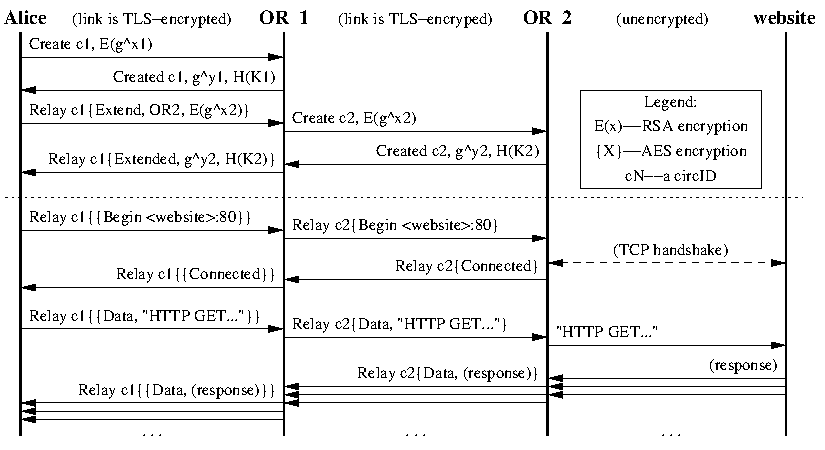
\includegraphics[width=0.9\textwidth]{pics/construction.pdf}
    \caption{Darstellung des Aufbaus und der Verwendung eines Circuits. Quelle: \cite{tor}}
    \label{fig:construction} 
  \end{center} 
\end{figure}

Wie in Abbildung \ref{fig:construction} nachvollzogen werden kann, hat sich der Extend Vorgang nicht geändert. Der Vorgang wurde lediglich vom Onion Proxy entfernt durch Relay Cells erledigt. Wichtig ist, dass der Schlüsselaustausch hier zwischen dem Onion Proxy und $\textit{OR}_2$ stattgefunden hat, $\textit{OR}_1$ hat die Daten lediglich weitergeleitet. Auch konnte $\textit{OR}_1$ keine Informationen gewinnen, da eine Hälfte des Schlüsselaustausches verschlüsselt wurde. Der Circuit ist nun um $\textit{OR}_2$ erweitert und der Onion Proxy und $\textit{OR}_2$ können nun mit $K_2$ wiederum verschlüsselte Relay Cells austauschen. Auf diese Weise können beliebig viele weitere Onion Router zu dem Circuit hinzugefügt werden.

\subsection{Cross Circuit Interference Problem.}
\label{sec:crosscircuitinterference} 

Unter den vielen Problemen die \textsc{Tor} bis heute noch hat, ist das Cross Circuit Interference Problem eines der konzeptuell schwerwiegensten \cite{tor_improvements}.
\textsc{Tor} leidet unter gewissen Umständen unter hohen Netzwerklatenzen.
Für alle Circuits, die über die Verbindung zwischen zwei Onion Router laufen, wird in \textsc{Tor} genau eine TCP-Verbindung verwendet.
Das führt dazu, dass alle Circuits dem selben TCP-Mechanismus zugrundeliegen.
Joel Reardon fand heraus, dass die Latenzen weder beim Empfangen noch vom Verarbeiten der Daten enstehen.
Er stellte fest, dass die Daten die meiste Zeit in den Output Buffern der TCP Implementierung warten und dass die Ursache für die Latenzen die TCP Congestion Control ist, welche Circuits mit niedriger Bandbreite im Vergleich zu Circuits mit hohem Durchsatz benachteiligt \cite{tcp-over-dtls-thesis,tcp-over-dtls}.

TCP garantiert eine fehlerfreie und Ordnung erhaltende Datenübertragung. Dazu wird jedes Paket, das vom Sender versendet wird, vom Empfänger bestätigt.
%Unbestätigte Pakete werden als ``unterwegs'' beziehungsweise ``On-the-fly'' angenommen, das bedeutet, dass sie noch im Netzwerk befinden.
Um unnötige Latenz zu vermeiden, wird dieser Prozess teils parallelisiert, das heißt, der Sender kann Pakete versenden bevor Bestätigungen der vorgehenden Pakete eingegangen sind. Dies muss jedoch begrenzt werden, da unter den bisherigen Bedingungen alle anstehenden Pakete versendet werden könnten, was das Netzwerk temporär überlasten würde.

Um die Last auf dem Netzwerk zu reduzieren wurde beim Sender ein sogenanntes \textit{Congestion Window} (CWND) zur Staukontrolle eingeführt. Das Congestion Window ist ein fiktives Fenster um die Reihe der zu versendenden Pakete, die ohne Bestätigung der Vorgänger versendet werden und somit parallel unterweges sein dürfen.

Teil des Congestion Control Mechanismus ist auch das Verwerfen von Paketen bei zu hoher Auslastung des Netzwerks. Nach einem festgelegten Timeout werden Pakete vom Sender als verworfen angenommen und neu versendet. An dieser Stelle wird nicht tiefer in die Details des Transmission Control Protocols eingegangen, mehr Informationen zum Handling des Congestion Windows und TCP generell kann in den relevanten RFCs gefunden werden \cite{rfc:tcp, rfc:tcpcc}.

\begin{figure}[h]
  \begin{center}
    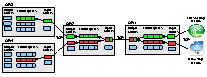
\includegraphics[width=0.8\textwidth]{pics/BufferPic.pdf}
    \caption{Beispielszenario in dem das Cross Circuit Interference Problem auftreten kann. Quelle: \cite{pctcp} }
    \label{fig:buffer} 
  \end{center} 
\end{figure} 

In Abbildung \ref{fig:buffer} wird ein Szenario dargestellt in dem der Fluss der Daten zweier Circuits über eine TCP-Verbindung vereint wird. Ein Circuit wird verwendet um eine Verbindung zu einer Webseite herzustellen und der andere Circuit wird verwedet um große Datenmengen mit der Filesharing Anwendung Bittorrent zu übertragen. Beide Circuits laufen Über OR1 und OR2. Bei der aktuellen \textsc{Tor}-Architektur bedeutet das, dass die beiden Circuits die TCP-Verbindung zwischen OR1 und OR2 und speziell die Aus- und Eingangspuffer im Kernelspace teilen. Unter Last kann das dazu führen, dass Circuits die relativ wenig Daten fördern, wie der Circuit zum Besuch der Webseite in dem obigen Szenario, verhältnismäßig große Latenzen haben.


Grund dafür ist das Head-on-line Blocking, welches entsteht wenn Pakete verloren gehen beziehungsweise bei Überlastung des Netzwerks verworfen werden. In diesem Fall setzt der Mechanismus der Staukontrolle ein. Der Sender erhält keine Bestätigung und die Pakete werden nach dem festgesetzten Timeout neu übertragen. Wie in Abbildung \ref{fig:headonline} zu sehen, werden Daten, die längst in Input Buffer zum lesen bereit sind, nicht freigegeben, weil auf ein bestimmtes, in der Sequenz vorhergehendes Paket gewartet wird. Da TCP für das erhalten der Ordnung des Datenstroms zuständig ist, dürfen die Pakete nicht an dei Anwendung weitergegeben werden. Der TCP Spezifikation entsprechend ist das erforderlich, für die Circuits in Tor ist das problematisch und nicht notwendig, da die Ordung schon auf der Streamebene erhalten wird.

\begin{figure}[h]
  \begin{center}
    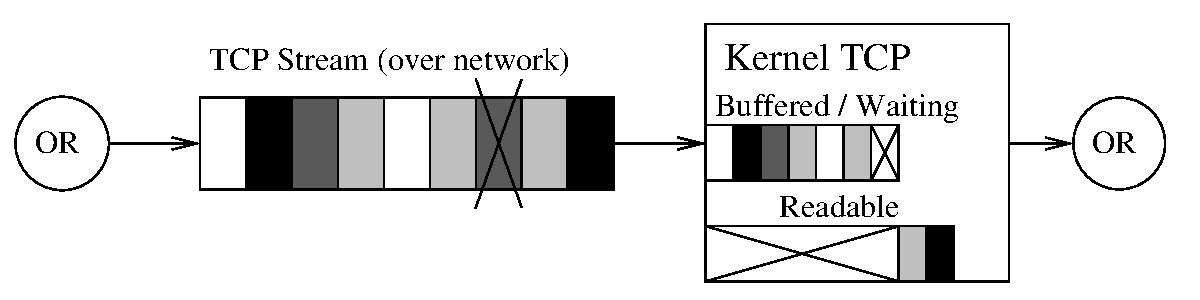
\includegraphics[width=0.7\textwidth]{pics/headonlinevanilla.pdf}
    \caption{Die unterschiedlich schattierten Rechtecke stellen Cells unterschiedlicher Circuits dar. Die letzten zwei Cells sind bereit zur Weitergabe an die Anwendung werden aber zurückgehalten. Quelle: \cite{tcp-over-dtls}}
    \label{fig:headonline} 
  \end{center} 
\end{figure}

%==============================================================================
\section{PCTCP}
\label{sec:pctcp}

In dem Artikel in dem Reardon auf diese Schwachstelle hinweist, schlagen die Autoren eine Lösungsansatz vor, in dem das Design dahingehend verändert wird, dass die für \textsc{Tor} unnötige Garantie die Ordung der Datenpakete zu erhalten umgangen wird. Das wir erreicht, indem für die Verbindungen zwischen den Onion Routern UDP-Verbindungen verwendet werden, worauf ein TCP Stack im Userspace aufsetzt. \cite{tcp-over-dtls}. Die Autoren nennen diesen Ansatz TCP-over-DTLS.

Im Detail bedeutet das, dass für die Verbindungen der einzelnen Circuits jeweils eine eigene TCP-Verbindung aufgebaut wird. Dadurch bleiben alle positiven Eigenschaften der vorherigen TCP-Verbindung erhalten und das Cross Circuit Interference Problem wird gelöst. Grund dafür ist, dass es nicht mehr vorkommen kann, dass mehrere Circuits dem Mechanismus der Staukontrolle einer einzigen TCP-Verbindung unterliegen. Somit besteht keine Möglichkeit der Interferenz mehr, da es in der selben TCP-Verbindung keine Cicuits mehr gibt auf die Einfluss genommen werden kann. Diese TCP-Verbindungen werden aber nicht vom Betriebsystem geöffnet. Nach dem Design des TCP-over-DTLS ist der TCP Stack Teil der \textsc{Tor}-Software. Die Pakete werden im Userspace erstellt und erst dann an das Betriebssystem weiter gegeben um per UDP beziehungsweise DTLS versendet zu werden. Datagram Transport Layer Security ist das UDP Äquivalent zu TLS für TCP \cite{dtls}. Es sorgt für die Vertraulichkeit und Authentizität auf der Strecke zwischen den einzelnen Onion Routern. Da im Vergleich zu TCP Sockets der UDP Socket nicht gebunden wird, reicht für den TCP-over-DTLS Ansatz genau ein Socket für beliebig vielen Verbindungen zu anderen Onion Routern aus.

Wenn ein Paket verworfen wird, dann wird lediglich die Staukontrolle eines bestimmten Circuits aktiviert, da die Circuits eigenes Congestion Window haben. Alle anderen bleiben unberührt und es kommt zu keiner Cross Circuit Interference. Siehe dazu die graphische Veranschaulichung in Abbildung \ref{fig:headonlinedtls}. Des weiteren werden die Pakete, wenn sie verworfen werden, gleichverteilt über den Datenstrom verworfen. Daraus folgt, dass die Wahrscheinlichkeit dass ein Paket verworfen wird, proportional zum Bandbreitenbedarf des Circuits auf der Verbindung steigt und somit die Fairness der Staukontrolle wieder hergestellt ist.

Die Lösung des TCP-over-DTLS scheint bestens geeignet, um die Latenzen im \textsc{Tor}-Netzwerk zu vermeiden. Die Autoren verwenden in ihrem Proof-of-concept allerdings die bereits vorhandene Userpace TCP Implementierung Daytona \cite{daytona}, aber in der Praxis gibt es leider keine Userpace TCP  Implementierung, deren Lizenz mit der des \textsc{Tor}-Projekts vereinbar ist. Daher entschied sich einer der Autoren, Ian Goldberg, einen alternativen Ansatz zu verfolgen, der auf dem selben ``Ein-Circuit-pro-TCP-Verbindung'' Prinzip des  TCP-over-DTLS aufbaut: das Per-Circuit TCP-over-IPsec. 

\begin{figure}[h]
  \begin{center}
    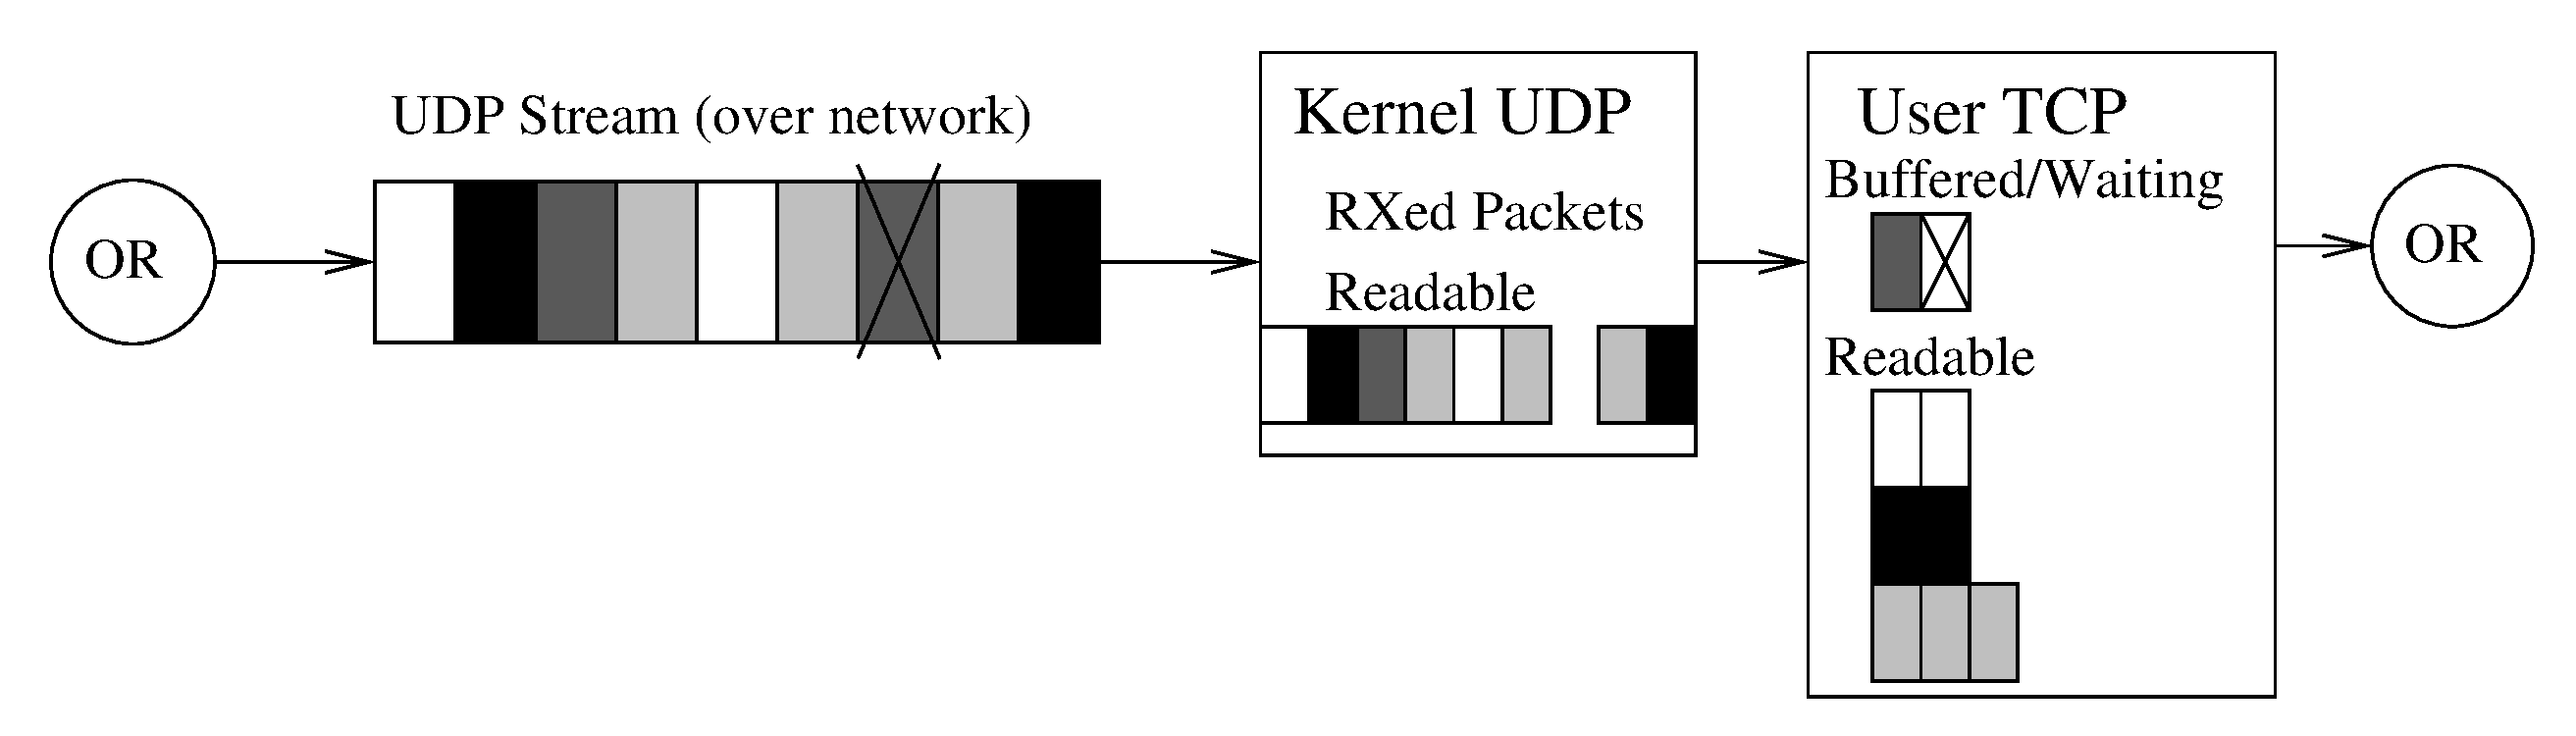
\includegraphics[width=0.7\textwidth]{pics/headonlinedtls.pdf}
    \caption{Die unterschiedlich schattierten Rechtecke stellen Cells unterschiedlicher Circuits dar. Alle empfangenen Cells werden nun an die Anwendung weitergegeben. Vergleiche Abbildung \ref{fig:headonline}. Quelle:\cite{tcp-over-dtls}}
    \label{fig:headonlinedtls} 
  \end{center} 
\end{figure} 

\subsection{Design}

PCTCP ist dem TCP-over-DTLS sehr ähnlich. Die Idee wie das Cross Circuit Interference Problem umgangen werden kann ist die selbe. Es wird ganz einfach für jeden Circuit eine neue TCP-Verbindung verwendet, damit die Staukontrolle nicht auf der Ebene der Verbindung zwischen je zwei Onion Router, sondern auf der Ebene der einzelnen Circuits läuft. Somit haben die Circuits keine Möglichkeit sich geegenseitig zu beeinflussen. Konzeptuell wurde das Multiplexing der Circuits also von der Transportschicht auf Vermittlungsschicht verschoben. Im Vergleich zum TCP-over-DTLS wird im PCTCP keine Userspace TCP-Verbindung, sondern eine übliche TCP-Verbindungen im Kernelspace, erstellt. Die Autoren sprechen hier von einer Kernel-Mode per-circuit TCP-Verbindung. 

Wenn ein Angereifer einen Onion Router überwacht könnte er so die einzelnen TCP-Ver\-bin\-dung\-en und somit Circuits zählen und den Datenverkehr analysieren, da die TCP-Header nicht verschlüsselt werden (Vgl. Abbildung \ref{fig:pctcpheader}). Daher wird die Onion Router zu Onion Router Verbindung per IPSec abgesichert.

Die Verbindung vom Onion Proxy zum ersten Onion Router wird wie gehabt zu erhalten. Es bleibt somit eine einzige TLS gesicherte Verbindung, über die alle Circuits gemutliplext werden, bestehen. Das bedeutet das die Cross Circuit Interference nicht ganz beseitigt wurde, hat aber den Vorteil, dass für die Umsetzung am Quelltext des Clients nichts geändert werden muss. Die Änderung des Designs findet lediglich im \textsc{Tor}-Netzwerk zwischen den Onion Routern statt. Die Netzwerkschnittstelle des PCTCP ist rückwartskompatibel zu Standard Tor Onion Routern. Das ermöglicht PCTCP inkrementell zu verteilen, da der Bertrieb eines herterogeneren Tor-Netzwerkes möglich ist.

\subsection{IPSec}

Internet Protocol Security (IPSec) ist eine Protollfamilie die Verbindungen über ein potentiell unsicheres Netzwerk sichert. IPsec soll in einem solchen Netzwerk die Schutzziele Vertraulichkeit, Authentizität und Integrität erhalten. Dazu bietet IPSec zwei Protokolle die in je zwei Modi betrieben werden können: IP Authentication Header \cite{rfc:ah} und IP Encapsulating Security Payload \cite{rfc:esp}.

Der IP Authentication Header (AH) erlaubt es den kommunizierenden Hosts die übertagenen Daten zu authentifizieren und die Integrität zu prüfen. Optional bietet es Features um Replayattacken zu verhindern. Allerdings kann es nicht für die Vertraulichkeit der Daten sorgen.

IP Encapsulating Security Payload (ESP) bietet ebenfalls Authentisierung und Integrität der übertagenen Daten. Zusätzlich können mit dem ESP die übertragenen Daten verschlüsselt werden, nachdem mit einem der Schlüsselaustauschverfahren, die auch Teil der IPsec Familie sind, ein gemeinsamer Schlüssel ausgehandelt wurde. 

Beide Protokolle können in zwei Modi betrieben werden: Dem Transport- und Tunnelmodus. Im Transportmodus wird die Verbindung zwischen zwei Hosts abgesichert. In diesem Modus sind die beiden Hosts die Endpunkte bezüglich der Kommunikation und Verschlüsselung. Das bedeutet das der Sender und Empfänger selbst für die Verschlüsselung und beziehungsweise oder Authentisierung der Daten zuständig sind. Da der Transport der Daten direkt von Host zu Host läuft, wird der IP Header weiterhin für das Routing benötigt. Der Rest, also ab der Transportschicht wird als Nutzlast des IPSec gefördert.

Im Tunnelmodus werden zwei Netzwerke durch einen IPsec-Tunnel verbunden. Dazu verbinden sich die Gateways zweier Netzwerke miteinander und die Internetzwerk Pakete werden über die IPSec Gateways geleitet. Die Pakete des Datenverkehrs werden von den Gateways samt IP Header gekapselt und mit einem neuen IP Header versehen. Der zusätzliche IP Header ist für das Routing zum gegenüberliegenden Gateway zuständig. Letzteres entpackt das empfangene Paket und leitet es in das eigene Netzwerk weiter. In diesem Modus sind die Endpunkte bezüglich der Verschlüsselung und Kommunikation nicht zwangsweise die selben Instanzen. Für die Sicherheit sind die Gateways zuständig, während die Kommunikationsendpunkte beliebige Teilnehmner aus den beiden Netzwerken sein können.

\begin{figure}[h]
  \begin{center}
    \begin{subfigure}[t]{0.46\textwidth}
      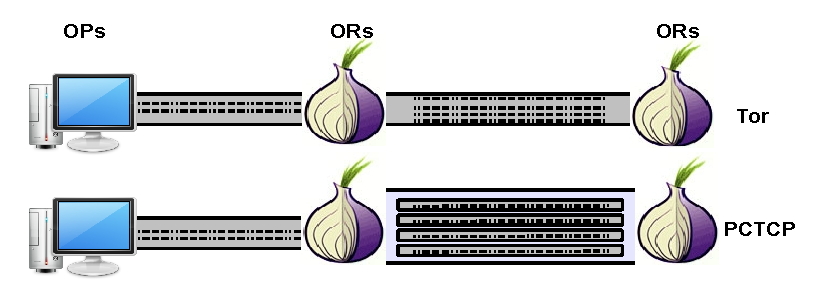
\includegraphics[width=\textwidth]{pics/PCTCP_design.pdf}
      \caption{Vergleich des Designs. Quelle: \cite{pctcp}}
      \label{fig:pctcpdesign}
    \end{subfigure}
    \begin{subfigure}[t]{0.46\textwidth}
      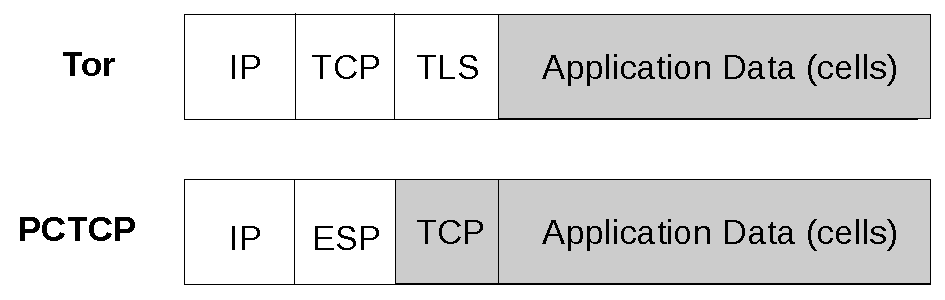
\includegraphics[width=\textwidth]{pics/PCTCP_header.pdf}
      \caption{Vergleich der Inter Onion Router Pakete. Grau schattierte Teile sind verschlüsselt. Quelle:\cite{pctcp}}
      \label{fig:pctcpheader}
    \end{subfigure}
    \caption{Vergleiche Zwischen Standard-\textsc{Tor} und PCTCP.}
  \end{center} 
\end{figure}

Da das ESP Protokoll alle Fähigkeiten des AH Protokolls und zusätzlich die für \textsc{Tor} wichtige Vertraulichkeit besitzt, wird für die Zwecke im PCTCP das ESP Protokoll verwendet. Zusätzlich würde das AH Protokoll ein praktisches Problem für \textsc{Tor} darstellen, da es nicht ohne weiteres mit NAT \footnote{Network Adress Translation \cite{rfc:nat} ist ein Verfahren, das die Netzwerkadressen in den  Headern der IP Pakete verändert, um mehrere Adressen auf eine abzubilden. Sinnvollerweise kommt dieser Mechanismus in Routern zum Einsatz und wird standardmäßig von den Internetgateways (Router) in Privathaushalten verwendet.}  vereinbar ist. Grund für die Inkompatibilität ist die Tatsache, dass das AH Protokoll die Integrität des IP Headers überwacht, welches aber während des Prozesses der Network Adress Translation geändert wird. Da \textsc{Tor} ein Netzwerk aus Freiwilligen ist und diese in den meisten Fällen vom Heimnetzwerk aus hinter einem Gateway mit NAT sind, kommt das AH Protokoll nicht in Frage und das ESP Protokoll wird für die Verbindungen verwendet.

Die Verbindungen die mit IPSec gesichert werden sollen, sind übliche Host-to-Host Verbindungen. Das bedeuet, dass die Hosts bezüglich der Verschlüsselung und Kommunikation Endpunkte sind. Folglich wird für die Zwecke des PCTCP das ESP Protokoll im Transport Mode verwendet.

\newpage Da IPSec im Transport Mode den TCP Header mitverschlüsselt, kann ein Überwacher eines Onion Routers die Verbindungen nicht mehr unterscheiden, und somit keine Verbindungen mehr zählen oder den Datenverkehr einzelner Verbindungen analysieren. Da das ESP Protokoll bereits für die Vertraulichkeit der Verbindungen sorgt, ist die Verschlüsselung der Verbindungen zwischen den Onion Routern durch SSL/TLS redundant und kann ausgelassen werden. Schliesslich vervollständigt sich das Bild des Designs, das die Autoren des PCTCP vorschlagen. Entsprechend der Namensgebung des Per-Circuit TCP-over-IPsec werden Verbindungen über \textsc{Tor}, die Circuits, in jeweils eigenen TCP-Verbindungen, welche über IPSec gesichert werden, erstellt. Eine graphische Darstellung des Designs befindet sich in Abbildung \ref{fig:pctcpdesign}.

\subsection{Circuit construction}

Wie auch im Standard \textsc{Tor} verbindet sich der Onion Proxy $\textit{OP}$ mit dem ersten Onion Router $\textit{OR}_1$ im \textsc{Tor}-Netzwerk mit einer einzigen TLS-Verbindung. Die beiden Kommunikationspartner haben einen symmetrischen Schlüssel ausgehandelt und können verschlüsselte Relay Cells austauschen. Um den Circuit um einen Onion Router $\textit{OR}_2$ zu erweitern, sendet $\textit{OP}$ eine Extend Relay Cell an $\textit{OR}_1$. Die Extend Relay Cell enthält die selben Informationen wie im Standard-\textsc{Tor}. Bis hierher gleicht der Prozess exakt dem Standard-\textsc{Tor} Verbindungsaufbau. Um jetzt eine Verbindung zu $\textit{OR}_2$ zu erstellen und somit den Circuit zu erweitern, erstellt $\textit{OR}_1$ in jedem Fall eine neue, IPSec gesicherte TCP-Verbindung zu $\textit{OR}_2$. Standard-\textsc{Tor} versucht hingegegen bestehende Verbindungen wieder zu verwenden. Das Verfahren läuft wie üblich weiter: $\textit{OR}_1$ sendet eine Create Control Cell an $\textit{OR}_2$, bekommt als Bestätigung eine Created Control Cell von $\textit{OR}_2$ zurück und verpackt diese in eine Extended Relay Cell und leitet sie weiter an $\textit{OP}$.

In Experimenten zeigten AlSabah und Goldberg, dass durch PCTCP eine 60 prozentige Verbesserung der Latenzen und circa 30 prozentige Verbesserung der Downloadzeiten erreicht werden konnten.
Die einzelnen Experimente und die genauen Ergebnisse sind in \cite{pctcp} einzusehen.

% Vorteile des Deployments (Funktion des heterogenen Netzwerks (Plain \textsc{Tor} + PCTCP)\\

%==============================================================================
\section{Diskussion}
\label{sec:discussion}

Die Verwendung von \textsc{Tor} bietet keine allumfassende Anonymität. Der Nutzer muss auf einen bewussten Umgang mit \textsc{Tor} achten. Es ist wichtig, dass er genau weiß inwiefern \textsc{Tor} Anonymität bietet und wo die Grenzen liegen. So kann sich der Nutzer zum Beispiel immernoch selbst durch sein Verhalten im Internet deanonymisieren. \textsc{Tor} bietet auch keine so genannte Protokoll Normalisierung, das heißt komplexe Protokolle aus höheren Schichten, wie zum Beispiel HTTP, können auch trotz der Verwendung von \textsc{Tor} Informationen über die Identität übertragen. Für diesen Dienst muss auf andere Mittel, wie zum Beispiel den Prokollfilter Privoxy, zurückgegriffen werden. \textsc{Tor} macht nicht mehr aber auch nicht weniger als die Anonymität auf der Vermittlungsschicht zu wahren.

Abgesehen vom Hauptziel seine Nutzer zu anonymisieren, unterliegt das Design von \textsc{Tor} weiteren Zielen. \textsc{Tor} sieht vor in der realen Welt auf eine einfache Weise eingesetzt werden zu können. Mögliche Hürden, zum Beispiel Kernelpatches oder vermeidbare manuelle Interkation, werden umgangen, so dass für den Benutzer die best mögliche Benutzerfreundlichkeit erreicht wird.Grund dafür ist die Tatsache, dass im Kontext von \textsc{Tor} die Benutzerfreundlichkeit in Korrelation zur Sicherheit steht. Die Benutzerfreundlichkeit beeinflusst direkt die Menge der Nutzer des Systems. In \textsc{Tor} werden die Benutzer hinter der Identität anderer Benutzer versteckt. Je weniger Nutzer also im Netzwerk teilmehmen, desto weniger Anonymität kann dem einzelnen Nutzer geboten werden.

Für die Arbeit an der Sicherheit definieren die Entwickler von \textsc{Tor} ein Bedrohungsmodell. Es wird angenommen, dass ein Angreifer Teile des Datenverkehrs im Netzwerk überwachen und Knotenpunkte kompromittieren oder selbst betreiben kann. Des weiteren ist er fähig Datenverkehr zu erstellen, modifizieren, verwerfen oder verzögern. In seinem Design bietet \textsc{Tor} keine Sicherheit gegen Ende-zu-Ende Attacken \cite{tor}. Wenn ein Angreifer es geschafft den Datenverkehr am Eingangs- und am Ausgangsknoten eines Circuits mitzuverfolgen, gilt die Anonymität als aufgedeckt. Diese Situation kann genutzt werden um mit Timing-Attacken und Datenverkehrsanalysen Verbindungen zu deanonymisieren.

\newpage Unter diesem Aspekt unterliegt PCTCP der Sicherheit des Standard Tor, denn die Einrichtung des IPSec benötigt Administratorrechte und muss manuell erledigt werden. Daraus folgt, dass für die freiwilligen Betreiber der Onion Router der Aufwand und die erforderliche technische Fachkompetenz für die Einrichtung letzterer erhöht wird. Durch die Steigerung der Hemmschwelle oder einfache durch mangelndes technisches Know-How sinkt die Zahl der freiwilligen Teilnehmner des Tor Netzwerkes. Folglich wird dadurch auch die allgemein gebotenen Anonymität verringert. Um diesen Effekt zu schmälern soll Tor mit Installationsskripten ausgeliefert werden. Ein weiterer Ansatz ist IPSec für den Nutzer transparent zu nutzen, indem es als Userspace Implementierung Teil der Tor Software wird.

%Inwiefern die mangelnde Zahl der Netzteilnehmer zur Gefahr für die Anonymität im Tor Netzwerk werden kann, zeigt die folgende Familie der Angriffe.

Die Lösung der Performanceprobleme durch PCTCP hat aber ihren Preis. Die Lösung des Cross Circuit Interference Problems wird erreicht, indem für jeden erstellten Circuit eine neue TCP-Verbindung geöffnet wird. Das führt für eine bestimmte Klasse der Angriffe zu einer extremen Effizienz\footnote{Tatsächlich ist das ``Per Circuit TCP``-Konzept nicht neu. Im Tor der ersten Generation wurde schon pro Circuit eine TCP Verbindung verwendet. Dieser Ansatz wurde aber in der zweiten Generation wegen der vielen teuren Public Key Operationen verworfen.\cite{tor}}: die Socket Exhaustion Angriffe. 

Sockets sind auf allen gängigen Betriebssystemen eine endliche Ressource. Um diese Grenze nicht zu erreichen begrenzt Tor die Verwendung der TCP Sockets intern. Dazu werden die stehenden Verbindungen mit einem Counter gezählt und wenn die Variable ConnLimit erreicht ist verweigert Tor neue Verbindungen zu öffnen. Auf Linuxsystemen liegt das Standardlimit des Betriebssystems bei 4096. Intern setzt Tor ConnLimit auf exakt den Wert den das Betriebsystem meldet. Unter Windows idt der Standard bei ca 16 Millionen angesiedelt. Mehr als ausreichend und Tor setzt daher ConnLimit hardcoded auf 15000 \cite{imux}.

Klassich konnte ein Angreifer schon immer eine Exit Node stillegen, indem er so viel wie möglich persistente Streams Netzwerk über eine bestimmte Exit Node leitet. Dadurch konnte der Angreifer aber nur Exit Nodes attackiern. Mit dem Sniper Angriff \cite{sniper} ist es möglich jeden beliebigen Onion Router im Netzwerk anzugreifen. Dazu wird ein Tor Circuit selbst über eine Tor Verbindung erstellt, wodurch der Angreifer anonym bleibt. Der anonyme Onion Proxy erstellt dann den Circuit über den anzugreifenden Knoten im Netzwerk. Das kostet den angegriffenen Onion Router effektiv einen Socket pro Onion Proxy Instanz, da im Standard Tor alle Circuits über eine TCP Verbindung gemultiplext werden. Somit mussten für diesen Angriff urspränglich so viele Onion Proxy Instanzen erstellt werden wie auf dem Zielknoten Sockets verbraucht werden sollten. Dieses Verahren ist schlecht skalierbar und für einen Angreifer wohl eher uninteressant.

Mit PCTCP werden die Socket Exhaustion Angriffe wesentlich einfacher. Um einen Knoten anzugreifen kann der Onion Proxy einen Teilcircuit bis zum Zielknoten erstellen und den Circuit zu einem beliebigen Onion Router erweitern. Da im PCTCP pro Circuit eine neue TCP Verbindung erstellt wird kann dem Zielknoten mit jedem Circuit der erstellt wird ein Socket geraubt werden. Dieser Vorgang wird nun so oft wiederholt, bis dem angegriffenen Onion Router die Sockets ausgehen.

Die Socket Exhaustion Angriffe haben alle das selbe Ziel: Auf dem Zielsystem sollen so viele Sockets verwendet werden, dass das System keine neuen Verbindungen mehr annehmen kann oder so sehr überlastet wird, dass die verwendeten Sockets nicht mehr verwendet werden können oder das Betriebsystem den Tor Prozess beendet. Mit einem Angriff auf einen Onion Router mit einem limitierten Sockets kann der Angreifer dafür sorgen, dass der Onion Router seinen Dienst nicht mehr ausüben kann. Er zwingt die Onion Proxies einen anderen Pfad für den Circuit zu wählen. Wenn der Onion Router diesen Angriff verhindern will, kann er das Limit aufheben. Allerdings bleibt der Onion Router trotzdem verwundbar, denn die Verbinungen kosten  Systemressourcen. So kann mit einer hohen Anzahl an Verbindungen erreicht werden, dass, durch Prozessor- oder Speicherauslastung, die Performance des Knoten sinkt oder der Prozess gar vom Systemkernel beendet wird. Wenn der Angreifer selbst Onion Router für Verkehrsanalysen betreibt, dann steigen seine Chancen somit, dass die neuen Pfade über Onion Router laufen. Ein weiter Grund warum die Größe des Netzwerkes respektive die Benutzerfreundlichkeit der Software direkt mit der Anonymität in Korrelation steht.

\section{Ausblick}

% Witzig weil die viel labern, aber im Prinzip gibts nur ein Problem.
% sonst schenken sich die Ansätze nichts großartig, im gegenteil

Pro:
\begin{itemize}
 \item Socket Exhaustion Angriffe betreffen auch TCP-over-DTLS
 \item (ABER! Userspace Tcp besser konfigurierbar ohne root)
 \item Wäre instant anwendbar
\end{itemize}
Contra:
\begin{itemize}
 \item Open Source Userspace IPSec gibt nicht genau so wie TCP Stack (TCP sogar noch eher)
 \item Kein Gewinn über  TCP-over-DTLS
 \item manuelle interaktion inakzeptabel 
\end{itemize}
Ergo: Weiterforschen! Vielleicht ist IMUX (intelligentes Kernel informed Socketmanagement) cool.



%==============================================================================


\bibliographystyle{splncs}
\bibliography{literatur}
%==============================================================================
\end{document}
